
\subsection{The experimental setting}

\paragraph{Database and computing power}

Throughout this section, we used the fastMRI database \cite{zbontar2018fastmri}. It contains MRI images of size $320\times 320$.
We focused on the single coil and fully sampled knee images.
The training set is composed of $973$ 3D volumes, which represents a total of $34~742$ slices. 
The validation set has $199$ volumes and $7135$ slices.

Some images in the dataset have a significant amount of noise. 
This presents three significant drawbacks: \rev{i) the high-frequency contents of the images is increased artificially promoting sampling schemes making it possible to reconstruct noise, ii) the signal-to-noise-ratio of the reconstructed images is decreased artificially and iii) we have shown that noise can dramatically impact the convergence of off-the-grid Fourier sampling optimization \cite{gossard2022spurious}.}
To mitigate these effects, we pre-processed all the slices using a non-local mean denoising algorithm \cite{buades2011non}.

The experiments are conducted on the Jean-Zay HPC facility. 
For each task we use $10$ cores and an Nvidia Tesla V100 with 16GB of memory.

\paragraph{Sampling}

The bounds of the constraint sets in \eqref{eq:constraint_sets} are given by:
\begin{equation}\label{eq:constraints}
    \alpha=\Delta t \gamma \frac{G_{max}}{K_{max}} \quad\text{ and }\quad \beta=\Delta t^2 \gamma \frac{S_{max}}{K_{max}},
\end{equation}
where $\Delta t$ is the sampling step of the scanner. Following \cite{chaithya2020}, we used the following realistic hardware constraints: $G_{max}=40$mT/m, $S_{max}=180$T/m/s, $K_{max}=2\pi$ and $\gamma=42.57$MHz/T. The value of $\Delta t$ is fixed to ensure that at maximal speed, the distance between two consecutive points equals the Shannon-Nyquist rate \cite{lazarus2020correcting}.

We consider two different scenarii: $25\%$ and $10\%$ undersampling.
Each shot consists of $646$ acquisition points and we use $N_s=40$ shots and $N_s=16$ shots respectively for the $25\%$ and the $10\%$ undersampling.
Each shot is constrained to start at the center of the k-space.
The first few points of each trajectory are fixed to be radial, see Appendix \ref{sec:handling_mass_0} for the technical details.

The family of densities is generated using the process described in Section~\ref{subsubsec:dengenerator} with $10^4$ densities generated at random.

\paragraph{Sampling baseline}

All the optimized schemes are compared to a state-of-the-art handcrafted baseline: the Sparkling method described in \cite{lazarus2019sparkling}. 
There, the attraction-repulsion problem \eqref{eq:discrepancy} is solved with a radial density $\rho$ \rev{constructed with a lot of care}.
Its value at the center has been optimized to yield the best possible signal-to-noise ratio on the validation set in a way similar to \cite{chaithya2021learning}.
The corresponding point configuration is given in Fig.~\ref{fig11} and Fig.~\ref{fig12} for the $25\%$ and $10\%$ undersampling rates respectively.
It provides a $7$dB improvement compared to the usual radial lines commonly found in the literature (see the first two rows of Table \ref{table:result_different_optim_TV}).

\paragraph{Image reconstruction}

The experiments are conducted with two reconstruction models:
\begin{itemize}
    \item a total variation reconstruction method with $120$ iterations of Algorithm~\ref{alg:TV_minimization} in Appendix~\ref{sec:reconstruction_algorithm_TV} and with a regularization parameter $\lambda=10^2$ and,
    \item an unrolled network (NN) with $6$ iterations of ADMM and a DruNet as the denoising step \cite{zhang2021plug}, $30$ iterations of the CG algorithm that initializes the ADMM and $10$ iterations of CG to solve the data-consistency equations at each iteration.
\end{itemize}
\rev{The parameter $\lambda$ was optimized to get the best mean square error for the baseline scheme and the number of iterations in the algorithms was chosen optimaly with respect to the reconstruction quality and the available memory on a GPU.}

\begin{figure*}[h!]
    \centering
    \plottraj{variablekernel_linear.pdf}
        {variablekernel_linear_zoom.pdf}
        {$h(x) = \|x\|_2$ --- $35.10$dB\\ $d(\xi)=0.52$}
        {0}
        {0}
        {0}{fig:dist:linear}{0}
    \hfill
    \begin{subfigure}[t]{.36\linewidth}
        \centering
        \includegraphics[width=\textwidth]{den14.png}
        \caption{Target radial density}
    \end{subfigure}
    \plottraj{variablekernel_log_a=1.pdf}
        {variablekernel_log_a=1_zoom.pdf}
        {$h(x)=\log(\|x\|_2)$ --- $35.35$dB\\ $d(\xi)=0.72$}
        {variablekernel_sqrt_a=1.pdf}
        {variablekernel_sqrt_a=1_zoom.pdf}
        {$h(x) = \sqrt{\|x\|_2}$ --- $35.32$dB\\ $d(\xi)=0.69$}{fig:dist:log1}{fig:dist:sqrt1}
    \caption{On the importance of the discrepancy's kernel $h(x)$. The same density is sampled with different kernels. The average PSNR of the reconstructed images on the validation set is displayed with its standard deviation. The average distance between contiguous points on the trajectories is displayed as $d(\xi)$.\label{fig:dist}}
\end{figure*}


\subsection{Choosing a kernel for the discrepancy}\label{subsec:kernel_discrepancy}

In all the previous ``Sparkling'' papers \cite{lazarus2019sparkling,chauffert2017projection}, the kernel function $h(x) = \|x\|_2$ was used. 
This choice seems like the most natural alternative since it is the only one which is scale invariant in the unconstrained setting. 
This means that if $\Xi = (\R^D)^M$ and if a density $\rho$ is dilated by a certain factor, then so is the optimal sampling scheme. 
However, this property is not true anymore when constraints are added. In that case, the choice of kernel turns out to be of importance. 

To illustrate this fact, we considered the three different radial kernels $h(x) = \|x\|_2$, $h(x) = \sqrt{\|x\|_2}$ and $h(x) = \log(\|x\|_2)$.
As can be seen on Fig. \ref{fig:dist}, performance variations of more than $0.2$dB in average  are obtained depending on the kernel. 
The reason is that contiguous points on the trajectories are spaced more or less depending on this choice. 
For instance, observe that the points on the zoom of Fig. \ref{fig:dist:linear} are more packed along the trajectories that on Fig. \ref{fig:dist:log1}.
To compensate for this higher longitudinal density, the sampler then increases the distance between adjacent trajectories, thereby creating holes in the sampling set. 
This is detrimental, since low frequency information is lost in the process.
This effect can be quantified by evaluating the distances between contiguous points in the k-space center. 
As can be seen, it goes from $0.52$ for the usual kernel $h(x)=\|x\|_2$ to a significantly higher value $0.72$ for the logarithmic kernel. The latter kernel creates a higher repulsion for neighboring points.


\begin{figure*}
    \centering
    \plottraj{init_traj_25.pdf}
        {init_traj_25_zoom.pdf}
        {Baseline radial 25\%}
        {init_traj_10.pdf}
        {init_traj_10_zoom.pdf}
        {Baseline radial 10\%}{fig11}{fig12}
    \plottraj{TV_BO_25.pdf}
        {TV_BO_25_zoom.pdf}
        {Bayesian density optimization 25\%}
        {TV_BO_10.pdf}
        {TV_BO_10_zoom.pdf}
        {Bayesian density optimization 10\%}{fig21}{fig22}
    \plottraj{TV_multiscale_25.pdf}
        {TV_multiscale_25_zoom.pdf}
        {Trajectory optimization 25\%}
        {TV_multiscale_10.pdf}
        {TV_multiscale_10_zoom.pdf}
        {Trajectory optimization 10\%}{fig31}{fig32}
    \caption{Optimized sampling schemes with various optimization approaches. A total variation reconstruction algorithm is used.\label{fig:trajectory_optim_TV}}
\end{figure*}


\subsection{Bayesian optimization: database size and numerical complexity}
\label{subsec:bayesian_optim_numerical}

In this section, we aim at evaluating the computational complexity of the Bayesian optimization routine. 
To this end, we study the impact of the number of images $K$ in the dataset, the size of the initial sampling set and the number of iterations, which are governing the algorithm's complexity.
\rev{Table~\ref{table:bo_results} and \ref{table:computational_time} summarize our main findings for the total variation reconstruction and unrolled neural network.}

\rev{In Table~\ref{table:bo_results}, we see that the number of images $K$ in the dataset has nearly no influence on the quality of the final sampling density.} 
Taking $K=32$ or $K=512$ images yields an identical PSNR on the validation set. This holds both for the 25\% and 10\% undersampling rates.
As can be seen in the Tables, reconstructing as little as $200\times 32$ images is enough to reach the best possible density in the family.
The same conclusion holds for the $10\%$ undersampling rate. This represents $18\%$ of a single epoch.

We also see that the initial sampling set of the convex $\Cc$ plays a marginal role on the quality of the final result. 
In addition, taking a small number of initial points allows \rev{us} to reduce the overall complexity of the algorithm to reach a given PSNR.

\rev{Finally, Table \ref{table:computational_time} allows us to conclude that taking a database of $32$ or $128$ images has only a marginal influence on the computing times (3 hours instead of 4 hours) of the Bayesian optimization routine. This feature is related to the fact that a significant amount of time is spent in the minimization of $\mathcal{L}$, whose numerical cost is independent of the number of images.
Hence, the fact that the algorithm seems to perform well for $32$ images is advantageous mostly when only small datasets can be generated.}

\begin{table}
    \small
    \centering
    \begin{tabular}{ccc|ccc}
        \toprule
        \rev{Recon.} & \makecell{$\#$ init. points} & \makecell{$\#$ evaluations} & \makecell{average PSNR\\$K=32$ images} & \makecell{average PSNR\\$K=128$ images} & \makecell{average PSNR\\$K=512$ images}  \\
        \midrule
        TV & $20$ & $200$ & \makecell{$35.64$dB} & \makecell{$35.65$dB} & \makecell{$35.65$dB} \\
        \midrule
        TV & $100$ & $300$ & \makecell{$35.63$dB} & \makecell{$35.66$dB} & \makecell{$35.66$dB} \\
        \midrule
        TV & $200$ & $300$ & \makecell{$35.65$dB} & \makecell{$35.66$dB} & \makecell{$35.66$dB} \\
        
        \toprule
        NN & $20$ & $200$ & \makecell{$38.14$dB} & \makecell{$38.10$dB} & \makecell{$38.09$dB} \\
        \midrule
        NN & $100$ & $300$ & \makecell{$38.17$dB} & \makecell{$38.05$dB} & \makecell{$38.08$dB} \\
        \midrule
        NN & $200$ & $300$ & \makecell{$38.20$dB} & \makecell{$38.08$dB} & \makecell{$38.10$dB} \\
        \bottomrule
    \end{tabular}
    \caption{Bayesian optimization on a convex set $\Cc$ of dimension $L=20$ using a total variation reconstruction algorithm and an unrolled network for $25\%$ undersampling. The PSNR is evaluated for the optimized density on the validation dataset containing $7135$ images. The total number of cost function evaluations is given in the second column. \label{table:bo_results}}
\end{table}



\subsection{Comparing optimization routines for the total variation reconstructor}\label{subsec:comparison_TV}

In what follows, we aim at comparing two different sampling optimization approaches:
\begin{description}
    \item[Trajectory optimization] The minimization of \eqref{eq:objective_xi} in the space of trajectories. We use a modified version of the multi-scale approach in \cite{wang2022b}, see Appendix \ref{sec:solving_xi}. 
    \item[BO density] The Bayesian approach to minimize \eqref{eq:objective_rho} globally. 
\end{description}
To compare these approaches, we conduct various experiments. The corresponding results are shown in Table~\ref{table:computational_time}, Table~\ref{table:result_different_optim_TV} and Fig~\ref{fig:trajectory_optim_TV}.
Below, we summarize our main findings.

\paragraph{Qualitative comparison of the sampling schemes}

In this paragraph, we compare our method with existing works \cite{wang2022b,weiss2021pilot}. 
The optimized sampling schemes are shown in Fig.~\ref{fig:trajectory_optim_TV} for the TV reconstructor.
In Fig.~\ref{fig:trajectory_optim_TV}, we see the results of the different optimization routines. 

The two optimization methods yield anisotropic sampling schemes with a higher density along the vertical axis.
However the trajectories present significant differences.

The Bayesian optimization yields a sampling scheme which covers the space more uniformly. 
The trajectories have a significantly higher curvature at the k-space center. 
These features are somehow hard-coded within the sampling generator $\Sc_M$ described in Section \ref{sec:sampler}.

The trajectory optimization yields trajectories which are locally linear and aligned at a distance of about a pixel.
This suggests that the trajectory optimization favors Shannon's sampling rate at the center of the k-space.
A potential explanation is as follows. When the sampling points are close to a subgrid \cite{gossard2022spurious}, the adjoint of the forward operator $A(\xi)^*$ is roughly the pseudo-inverse. 
Using a points configuration close to a subgrid therefore helps iterative reconstruction algorithms to converge.

Finally, at the bottom-left of the zoomed region on the 25\% undersampling rate, it seems that Bayesian optimization (Fig.~\ref{fig21}) yields a density slightly higher  than trajectory optimization (Fig.~\ref{fig31}). 
This density is critical for the reconstruction quality and might explain a part of the quantitative differences observed in the next section.


\begin{table}[h!]
    \centering
    \small
    \begin{tabular}{lcc}
    \toprule
    Method & Computational time TV & \rev{Computational time NN}  \\ [0.5ex]
    \midrule
    Trajectory optimization & $85$h & \rev{$97$h} \\
    \rev{14 epochs} & \\
    \hline
    Bayesian optimization &  \\
    \hspace{0.4cm}Optimization $K=32$ & $3$h  & \rev{$4$h} \\
    \hspace{0.4cm}Optimization $K=128$ & $4$h & \rev{$5$h} \\
    \bottomrule
    \end{tabular}
    \caption{Computational time of the different optimization procedures ($25\%$ undersampling) with an NVIDIA Quadro RTX 5000 GPU.}
    \label{table:computational_time}
\end{table}

\paragraph{Performance comparison}

Table~\ref{table:result_different_optim_TV} reveals that the trajectory optimization yields better performance \rev{in average} than the Bayesian optimization approach both for the 25\% ($+0.26$dB) and 10\% ($+0.07$dB) undersampling rates.
This was to be expected since the density optimization is much more constrained.
The difference is however mild.

\rev{In Fig.~\ref{fig:sample_best_worst_TV}, we display some images which benefited the least (resp. the most) from the sampling scheme optimization, with respect to the baseline. For the total variation reconstructor, some images actually suffer from the sampling scheme optimization as can be seen on the left of the picture. However, they correspond to slices which are not dominant in the dataset. On the other hand, the images that benefit the most from trajectory optimization correspond to central slices, prevalent in the set. As for the neural network, the best increases are obtained with the outer slices, which could be due to the large constant areas, the network is able to reproduce easily. Finally, the largest decreases for the neural network as a reconstruction mapping are not clearly associated to a specific type of slice.}

\begin{table}
    \centering
    \small
    \begin{tabular}{>{\raggedright\arraybackslash}p{9em} >{\centering\arraybackslash}p{12em} >{\centering\arraybackslash}p{12em}}
    \toprule
    Method & $25\%$ & $10\%$ \\ [0.5ex]
    \midrule
    Radial scheme & \makecell{$27.87$dB \\ $0.66$} & \makecell{$24.28$dB \\ $0.57$} \\
    \hline
    Sparkling radial (baseline) & \makecell{$35.35$dB \\ $0.85$} & \makecell{$32.94$dB \\ $0.79$} \\
    \hline
    Bayesian optim. $K=128$ & \makecell{$35.66$dB ($+0.31$) \\ $0.86$} & \makecell{$33.41$dB ($+0.47$) \\ $0.80$} \\
    \hline
    Trajectory optim. $K=34742$ & \makecell{$35.92$dB ($+0.57$) \\ $0.87$} & \makecell{$33.48$dB ($+0.54$) \\ $0.80$} \\
    \hline
    Trajectory optim. $K=32$ & \makecell{$35.67$dB ($+0.32$) \\ $0.86$} & \makecell{$32.84$dB ($-0.10$) \\ $0.79$} \\
    \hline
    Trajectory optim. $K=128$ & \makecell{$35.67$dB ($+0.32$) \\  $0.86$} & \makecell{$32.89$dB ($-0.05$) \\ $0.79$} \\
    \bottomrule
    \end{tabular}
    \caption{Comparison of different optimization procedures for the TV reconstructor with different numbers of images $K$ in the training set. For each test case, the first line is the PSNR and the second line is the SSIM. \rev{We added the gain in PSNR with respect to the baseline in parentheses.} \label{table:result_different_optim_TV}}
\end{table}

\paragraph{Computing times}

Table~\ref{table:computational_time} gives the computation times for each method with the total variation reconstruction method.
The proposed approach has the significant advantage of giving an optimized sampling scheme with guarantees on the underlying density with a reduced computational budget and with a reduced number of images.
As can be seen, our approach requires only $32$ images and 3 hours.
This has to be compared to the 85 hours (3 days and a half) needed by the trajectory optimization routine.

This feature is a significant advantage of our approach. 
It could be key element when targeting high resolution images or 3D data.


\paragraph{Size of the training set}

As advertised, the Bayesian optimization approach works even for small datasets.
The trajectory optimization routine also  provides competitive results with only $32$ images in the training set. 
However, the performance collapses for the $10\%$ undersampling rate. 
Increasing the size of the training set to $K=128$ does not improve the situation.
This feature is in strong favor of our approach, when having access to a limited dataset.

\begin{figure*}[htbp]
    \centering
    \begin{tabular}{c ccc c ccc}
        & \multicolumn{7}{c}{
            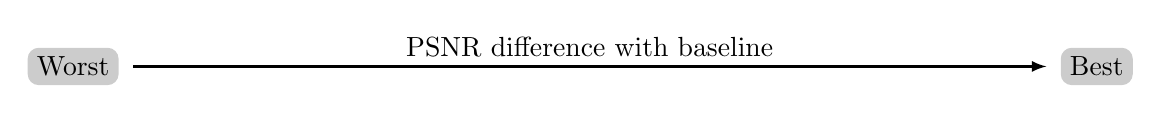
\begin{tikzpicture}
                \node[rounded corners=4pt,fill=black!20] (W) at (0,0) {Worst};
                \node[rounded corners=4pt,fill=black!20] (B) at (13,0) {Best};
                \draw[->,>=latex,thick,shorten >=5pt,shorten <=5pt] (W) -- (B) node[midway,above,rounded corners=4pt]{PSNR difference with baseline} ;
            \end{tikzpicture} 
        } \\

        \rotatebox[origin=l]{90}{BO TV} &
        \begin{subfigure}[t]{0.12\textwidth}
            \centering
            \includegraphics[width=\textwidth]{TV_40_bo_worst_orig_6.png}
            \caption*{$-1.3$dB}
        \end{subfigure} &
        \begin{subfigure}[t]{0.12\textwidth}
            \centering
            \includegraphics[width=\textwidth]{TV_40_bo_worst_orig_1.png}
            \caption*{$-1.1$dB}
        \end{subfigure} &
        \begin{subfigure}[t]{0.12\textwidth}
            \centering
            \includegraphics[width=\textwidth]{TV_40_bo_worst_orig_2.png}
            \caption*{$-1.1$dB}
        \end{subfigure} &
        \begin{tikzpicture}
            \draw[color=white](0,0) rectangle (0.2,1.5);
            \draw[color=black](0,0.8) node{$\hdots$};
        \end{tikzpicture}   &
        \begin{subfigure}[t]{0.12\textwidth}
            \centering
            \includegraphics[width=\textwidth]{TV_40_bo_best_orig_3.png}
            \caption*{$+1.4$dB}
        \end{subfigure} &
        \begin{subfigure}[t]{0.12\textwidth}
            \centering
            \includegraphics[width=\textwidth]{TV_40_bo_best_orig_5.png}
            \caption*{$+1.4$dB}
        \end{subfigure} &
        \begin{subfigure}[t]{0.12\textwidth}
            \centering
            \includegraphics[width=\textwidth]{TV_40_bo_best_orig_7.png}
            \caption*{$+1.4$dB}
        \end{subfigure} \\

        \rotatebox[origin=l]{90}{TO TV} &
        \begin{subfigure}[t]{0.12\textwidth}
            \centering
            \includegraphics[width=\textwidth]{TV_40_multi_worst_orig_9.png}
            \caption*{$-1.4$dB}
        \end{subfigure} &
        \begin{subfigure}[t]{0.12\textwidth}
            \centering
            \includegraphics[width=\textwidth]{TV_40_multi_worst_orig_7.png}
            \caption*{$-0.9$dB}
        \end{subfigure} &
        \begin{subfigure}[t]{0.12\textwidth}
            \centering
            \includegraphics[width=\textwidth]{TV_40_multi_worst_orig_1.png}
            \caption*{$-0.7$dB}
        \end{subfigure} &
        \begin{tikzpicture}
            \draw[color=white](0,0) rectangle (0.2,1.5);
            \draw[color=black](0,0.8) node{$\hdots$};
        \end{tikzpicture}   &
        \begin{subfigure}[t]{0.12\textwidth}
            \centering
            \includegraphics[width=\textwidth]{TV_40_multi_best_orig_1.png}
            \caption*{$+1.6$dB}
        \end{subfigure} & 
        \begin{subfigure}[t]{0.12\textwidth}
            \centering
            \includegraphics[width=\textwidth]{TV_40_multi_best_orig_5.png}
            \caption*{$+1.7$dB}
        \end{subfigure} &
        \begin{subfigure}[t]{0.12\textwidth}
            \centering
            \includegraphics[width=\textwidth]{TV_40_multi_best_orig_9.png}
            \caption*{$+1.8$dB}
        \end{subfigure} \\

        \rotatebox[origin=l]{90}{BO NN} &
        \begin{subfigure}[t]{0.12\textwidth}
            \centering
            \includegraphics[width=\textwidth]{NN_BO_worst_0_-1.3.png}
            \caption*{$-1.3$dB}
        \end{subfigure} &
        \begin{subfigure}[t]{0.12\textwidth}
            \centering
            \includegraphics[width=\textwidth]{NN_BO_worst_1_-1.1.png}
            \caption*{$-1.1$dB}
        \end{subfigure} &
        \begin{subfigure}[t]{0.12\textwidth}
            \centering
            \includegraphics[width=\textwidth]{NN_BO_worst_2_-1.1.png}
            \caption*{$-1.1$dB}
        \end{subfigure} &
        \begin{tikzpicture}
            \draw[color=white](0,0) rectangle (0.2,1.5);
            \draw[color=black](0,0.8) node{$\hdots$};
        \end{tikzpicture}   &
        \begin{subfigure}[t]{0.12\textwidth}
            \centering
            \includegraphics[width=\textwidth]{NN_BO_best_2_4.8.png}
            \caption*{$+4.8$dB}
        \end{subfigure} & 
        \begin{subfigure}[t]{0.12\textwidth}
            \centering
            \includegraphics[width=\textwidth]{NN_BO_best_3_4.9.png}
            \caption*{$+4.9$dB}
        \end{subfigure} &
        \begin{subfigure}[t]{0.12\textwidth}
            \centering
            \includegraphics[width=\textwidth]{NN_BO_best_4_5.3.png}
            \caption*{$+5.3$dB}
        \end{subfigure} \\

        \rotatebox[origin=l]{90}{TO NN} &
        \begin{subfigure}[t]{0.12\textwidth}
            \centering
            \includegraphics[width=\textwidth]{NN_TO_worst_0_0.1.png}
            \caption*{$0.1$dB}
        \end{subfigure} &
        \begin{subfigure}[t]{0.12\textwidth}
            \centering
            \includegraphics[width=\textwidth]{NN_TO_worst_1_0.3.png}
            \caption*{$0.3$dB}
        \end{subfigure} &
        \begin{subfigure}[t]{0.12\textwidth}
            \centering
            \includegraphics[width=\textwidth]{NN_TO_worst_2_0.3.png}
            \caption*{$0.3$dB}
        \end{subfigure} &
        \begin{tikzpicture}
            \draw[color=white](0,0) rectangle (0.2,1.5);
            \draw[color=black](0,0.8) node{$\hdots$};
        \end{tikzpicture}   &
        \begin{subfigure}[t]{0.12\textwidth}
            \centering
            \includegraphics[width=\textwidth]{NN_TO_best_2_5.1.png}
            \caption*{$+5.1$dB}
        \end{subfigure} & 
        \begin{subfigure}[t]{0.12\textwidth}
            \centering
            \includegraphics[width=\textwidth]{NN_TO_best_3_5.2.png}
            \caption*{$+5.2$dB}
        \end{subfigure} &
        \begin{subfigure}[t]{0.12\textwidth}
            \centering
            \includegraphics[width=\textwidth]{NN_TO_best_4_5.8.png}
            \caption*{$+5.8$dB}
        \end{subfigure}
    \end{tabular}
    \caption{\rev{PSNR differences between the optimized sampling schemes and the baseline for different images. The images were sorted with increasing PSNR differences from the left to the right. BO corresponds to the result with Bayesian optimization and TO corresponds to trajectory optimization. TV correponds to a total variation reconstruction and NN to an unrolled ADMM reconstruction. In this experiment, we used sampling schemes with $25\%$ undersampling. The numbers below the images are the PSNR differences between the baseline sampling scheme and the optimized trajectories.}}
    \label{fig:sample_best_worst_TV}
\end{figure*}


\subsection{Comparing optimization routines for a neural network reconstructor}\label{subsec:comparison_NN}

The aim of this section, is to compare three different sampling optimizers:
\begin{itemize}
    \item The Bayesian density optimization solver proposed in this paper. 
    \item The trajectory optimization solver with a fixed unrolled neural network trained on a family of sampling schemes, see Appendix \ref{sec:training_on_family}. 
    This is a novelty of this paper. 
    \item An optimization routine minimizing the trajectories and the unrolled network weights simultaneously, as proposed in \cite{wang2022b,weiss2021pilot}.
\end{itemize}

\paragraph{Qualitative comparisons}

The differences between the density optimization and the trajectory optimization can be observed on Fig. \ref{fig:optimmultiNN}. 
They are much more pronounced than for the total variation reconstructor. 
Surprisingly, the trajectory optimized sampling schemes leave large portions of the low frequencies unexplored.
Hence, it seems that the unrolled network is able to infer low frequency information better than the traditional total variation prior.
This suggests that the existing compressed sampling theories designed for the Fourier-Wavelet system have to be revised significantly to account for the progress in neural network reconstructions. 
The optimization of a trajectory for a fixed sampling scheme or the joint optimization yield qualitatively similar trajectories, with perhaps larger unexplored parts of the k-space for the fixed reconstruction method. 

\paragraph{Quantitative comparisons}

\begin{table}
    \centering
    \small
    \begin{tabular}{>{\raggedright\arraybackslash}p{12em} >{\centering\arraybackslash}p{12em} >{\centering\arraybackslash}p{12em}}
    \toprule
    Method & $25\%$ & $10\%$ \\ [0.5ex]
    \midrule
    Baseline with unrolled net & \makecell{$37.26$dB \\ $0.89$} & \makecell{$34.49$dB \\ $0.83$} \\
    \hline
    BO scheme $K=128$ with unrolled net & \makecell{$38.20$dB ($+0.94$) \\ $0.91$} & \makecell{$35.13$dB ($+0.64$) \\ $0.86$} \\
    \hline
    Traj. optim. with fixed unrolled net \rev{$K=34742$} & \makecell{$39.09$dB ($+1.83$) \\ $0.92$} & \makecell{$35.65$dB ($+1.16$) \\ $0.85$} \\
    \hline
    Joint optim. multi-scale \rev{$K=34742$} & \makecell{$39.03$dB ($+1.77$) \\ $0.92$} & \makecell{$35.53$dB ($+1.04$) \\ $0.85$} \\
    \bottomrule
    \end{tabular}
    \caption{Comparison of different optimization procedures for the unrolled ADMM reconstructor. For each test case, the first line is
the PSNR and the second line is the SSIM. \rev{The increase in PSNR compared to the baseline scheme is shown in parentheses}.\label{table:result_different_optim_NN}}
\end{table}
Table~\ref{table:result_different_optim_NN} allows  comparing the different methods quantitatively.
BO yields a PSNR increase almost twice lower than the multi-scale optimization (+0.94dB VS +1.83dB for 25\% and +0.64dB VS +1.16dB for 10\%).
This can likely be explained by the fact that the chosen family of densities (dimension 20) is unable to reproduce the complexity of the optimized trajectories.
It is possible that richer sampling densities could reduce the gap between both approaches.
However, Bayesian optimization is known to work only in small dimension and it is currently unclear how to extend the method to this setting. 

Interestingly, the trajectory optimized with a fixed unrolled neural network trained on a family provides slightly better results ($\approx +0.1$dB) than the joint optimization.
This suggests that the joint optimization gets trapped in a local minimizer since it can only be better if optimized jointly with the reconstructor.



\begin{figure*}
    \centering
    \plottraj{NN_BO_25.pdf}
        {NN_BO_25_zoom.pdf}
        {Bayesian density optim. $25\%$}
        {NN_BO_10.pdf}
        {NN_BO_10_zoom.pdf}
        {Bayesian density optim. $10\%$}{}{}
    \plottraj{NN_multiscale_dn_25.pdf}
        {NN_multiscale_dn_25_zoom.pdf}
        {Joint traj. optim. $25\%$}
        {NN_multiscale_dn_10.pdf}
        {NN_multiscale_dn_10_zoom.pdf}
        {Joint traj. optim. $10\%$}{}{}
    \plottraj{NN_multiscale_dn_fixed_25.pdf}
        {NN_multiscale_dn_fixed_25_zoom.pdf}
        {Traj. optim. with fixed net $25\%$}
        {NN_multiscale_dn_fixed_10.pdf}
        {NN_multiscale_dn_fixed_10_zoom.pdf}
        {Traj. optim. with fixed net $10\%$}{}{}
    \caption{Optimized sampling schemes with the various optimization approaches for a neural network reconstruction.}
    \label{fig:optimmultiNN}
\end{figure*}